\documentclass[11pt,a4paper]{article}
\usepackage[utf8]{inputenc}
\usepackage[german]{babel}
\usepackage{amsmath}
\usepackage{amsfonts}
\usepackage{subfig}
\usepackage{amssymb}
\usepackage{siunitx,physics}
\usepackage{mathtools}
\usepackage{graphicx}
%\usepackage{Here}
\usepackage[version=4]{mhchem}
\usepackage{url}
\usepackage{setspace}
\usepackage[left=2.5cm,right=2.5cm,top=2.5cm,bottom=2cm]{geometry}
[biblography=totocnumbered]
\usepackage{fancyhdr}
\usepackage{scrextend}
\usepackage{hyperref}
\pagenumbering{gobble}

\makeatletter
\newcommand\bigcdot{\mathpalette\bigcdot@{.5}}
\newcommand\bigcdot@[2]{\mathbin{\vcenter{\hbox{\scalebox{#2}{$\m@th#1\bullet$}}}}}
\makeatother

\makeatletter
%\renewcommand*\bib@heading{%
%  \subsection*{}%
%  \@mkboth{\refname}{\refname}}
%\makeatother
\numberwithin{equation}{section}
\numberwithin{figure}{section}

\renewcommand{\labelitemii}{\labelitemfont$\vartriangleright$}
\begin{document}\\
\begin{addmargin}[25pt]{0pt}
Man kann zum Einen das Kriechexperiment durchführen, dabei wird stufenartig eine Spannung angelegt und die Dehnung in Abhängigkeit von der Zeit beobachtet, die erwarteten Dehnungsantworten von elastischen, viskoelastischen und viskosen Materialien sind in Abbildung \ref{fig:Kriechexperiment} dargestellt.
\begin{figure}[h]
    \centering
    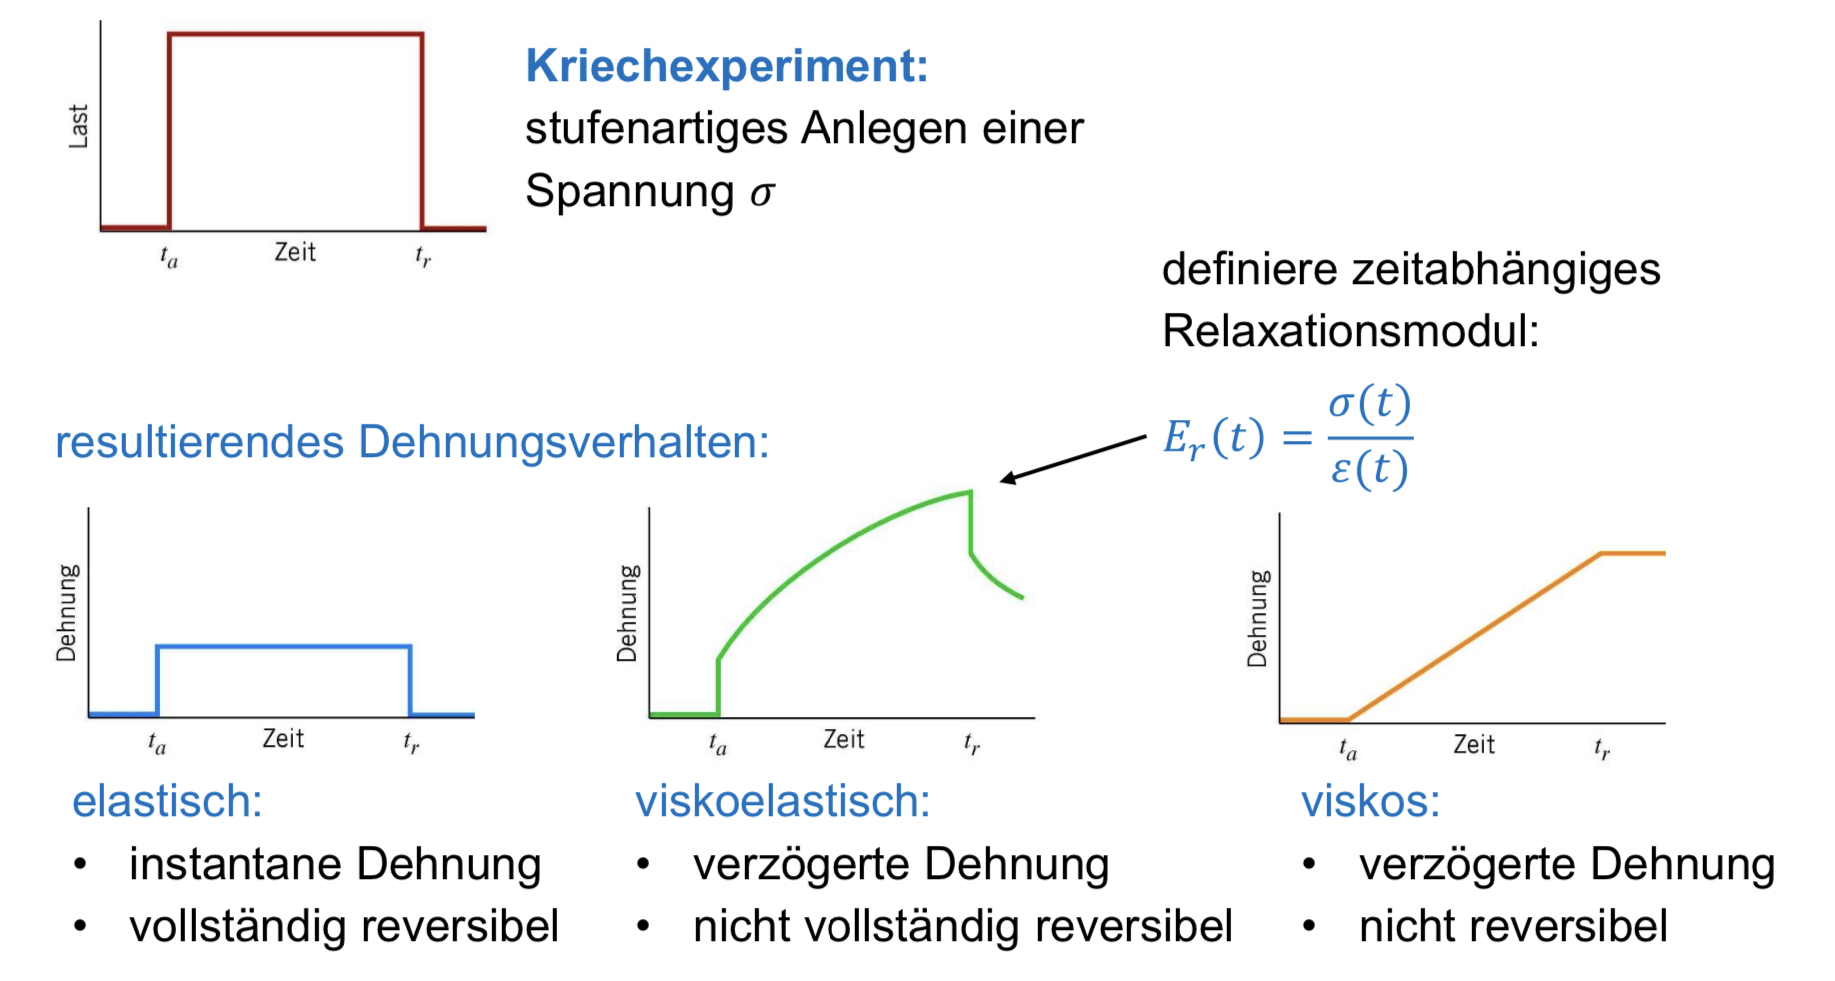
\includegraphics[width = \textwidth]{images/Materialwissenschaften/Kriechexperiment.jpeg}
    \caption{Verschiedene Dehnungsantworten auf eine stufenartige Spannung im Kriechexperiment}
    \label{fig:Kriechexperiment}
\end{figure}
Zum Anderen kann man das Relaxationsexperiment durchführen, dabei wird eine stufenartige Dehnung angelegt und die Spannungsantwort des Materials beobachtet, typische Spannungsantworten sind in Abbildung \ref{fig:Relaxationsexperiment} dargestellt.
\begin{figure}[h]
    \centering
    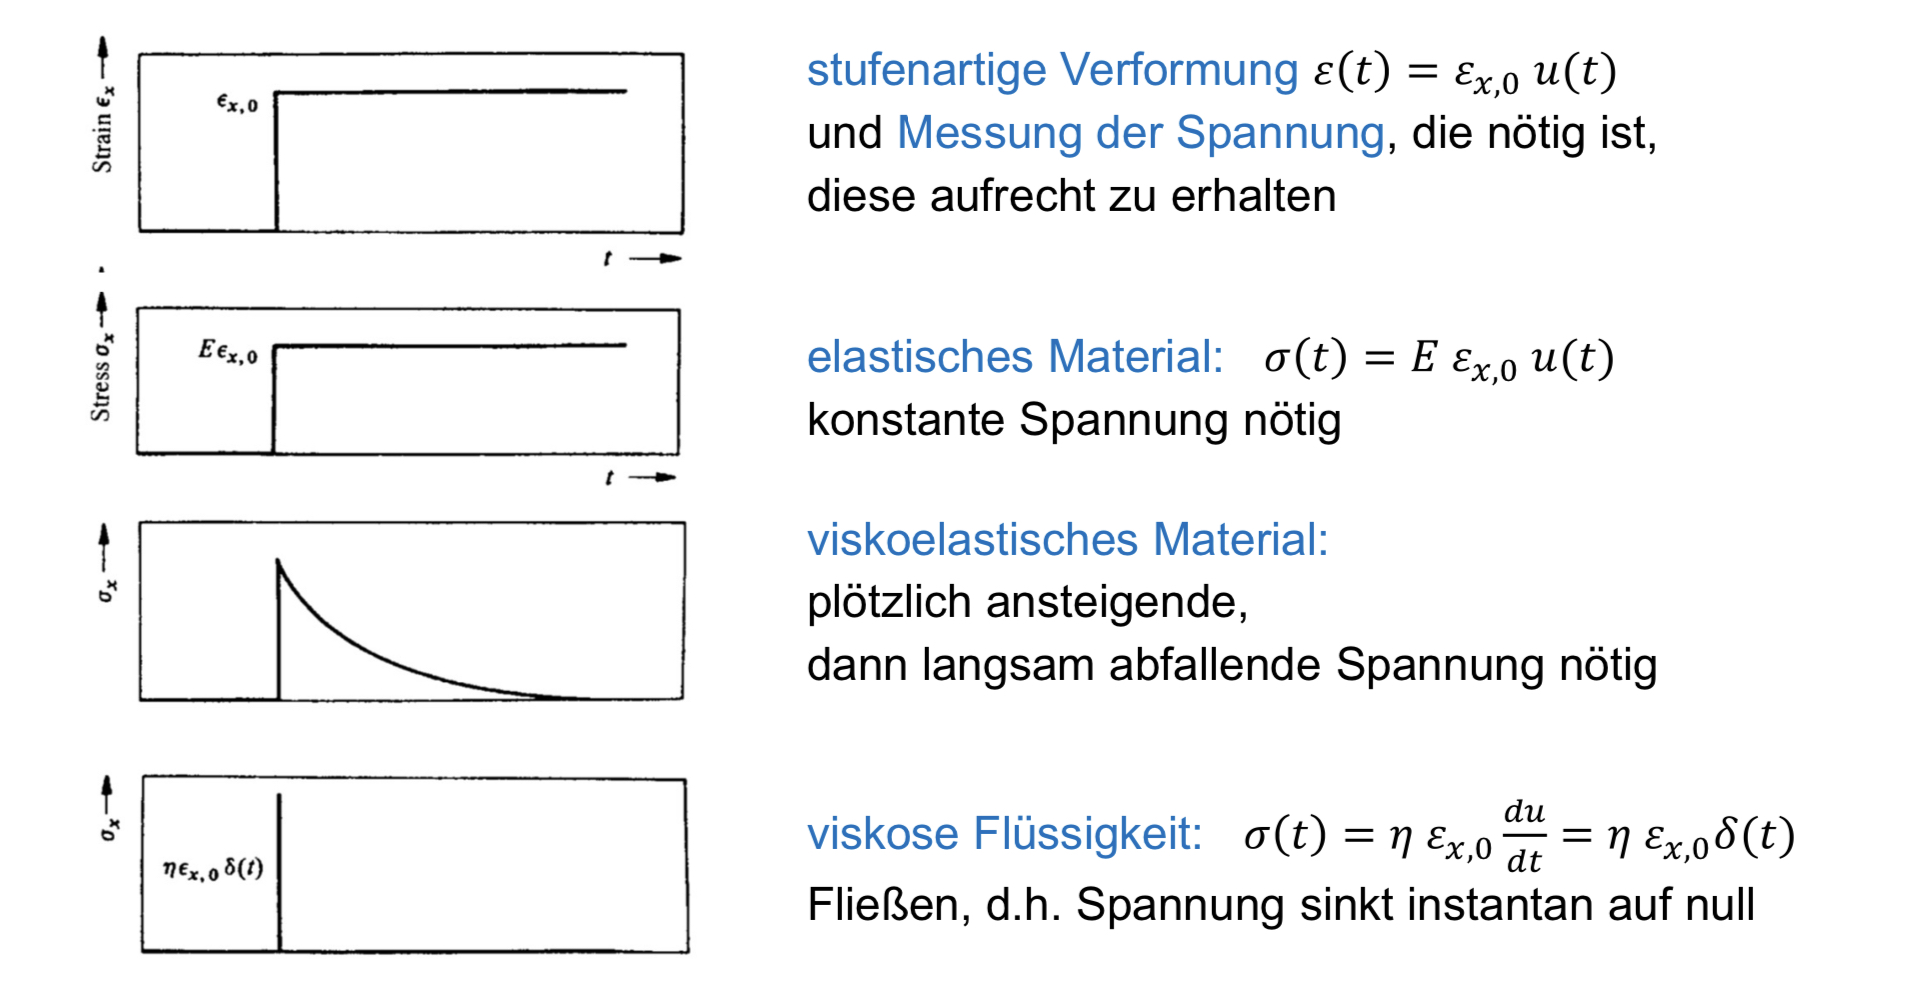
\includegraphics[width = 0.8\textwidth]{images/Materialwissenschaften/Relaxationsexperiment.jpeg}
    \caption{Verschiedene Spannungsantworten auf eine stufenartig angelegte Dehnung im Relaxationsexperiment}
    \label{fig:Relaxationsexperiment}
\end{figure}
\end{addmargin}

\end{document}